\section{Development Environment Configuration}

In software development, creating a reproducible and isolated development
environment is essential for ensuring consistency across different systems
and developers. This section discusses how to utilize two key technologies for
setting up such environments: functional package management and containerization.
The goal is to create development environments that are isolated from the host
system, ensuring consistency in the development process regardless of the
developer's operating system or machine configuration.

The following subsections will discuss each approach in detail, starting with
functional package management and its role in setting up development environments.

\subsection{Functional Package Management for Development Environments}

In a functional package management system, such as Nix, developers can define their
entire development environment, including compilers, libraries, tools, and other
dependencies, in a single configuration file. This file describes the precise
version of every component needed for development and testing.

Below is an example of how this can be achieved using a configuration file. While
the following implementation is specific to Nix, the concepts are general and can
be applied to other functional package management systems. The file defines inputs,
which include external resources like package repositories and overlays for specific
languages or tools.

\begin{lstlisting}[caption={Input section for functional package management}]
{
  inputs = {
    nixpkgs.url = "github:NixOS/nixpkgs/nixos-unstable";
    flake-utils.url = "github:numtide/flake-utils";
    nix-filter.url = "github:numtide/nix-filter";
    rust-overlay = {
      url = "github:oxalica/rust-overlay";
      inputs.nixpkgs.follows = "nixpkgs";
    };
  };
\end{lstlisting}

In this example, the inputs define the external sources required to build the
environment. The main idea is that the package repository (here represented by
nixpkgs) and overlays (such as rust-overlay) provide packages in a purely
functional manner, ensuring that different versions of packages can coexist without
conflicts. The configuration guarantees that the exact same packages will be
used by all developers working on the project.

The outputs section defines what is produced by the functional package management
system, including development shells. A development shell is an isolated environment
that includes all the tools and dependencies needed for development. By defining
such environments declaratively, functional package managers ensure that all
developers have access to the same setup.

\begin{lstlisting}[caption={Outputs section for functional package management}]
  outputs = inputs:
    with inputs;
      flake-utils.lib.eachDefaultSystem (
        system: let
          inherit (nixpkgs) lib;
          overlays = [(import rust-overlay)];
          filter = nix-filter.lib;
          pkgs = import nixpkgs { inherit system lib overlays; };
          bin = pkgs.pkgsBuildHost.rust-bin;
          rustToolchain = bin.fromRustupToolchainFile ./rust-toolchain.toml;
\end{lstlisting}

The outputs are built in a way that respects the functional programming paradigm.
This means that each output is a pure function of its inputs, and any change in the
input will result in a predictable change in the output. For example, a change in
the rust-overlay version will result in a new environment that reflects that
specific version of Rust, without affecting other environments that rely on a
different version.

Functional package management systems also allow the definition of development
shells, which are isolated environments that provide all the tools and dependencies
needed for development. These shells are constructed based on the inputs and outputs
defined in the configuration file.

\begin{lstlisting}[caption={Development shell for functional package management}]
            devShells = {
              default = mkShell {
                buildInputs = [pkg-config];
                nativeBuildInputs = [
                  extendedRustToolchain
                  rust-analyzer
                  openssl
                  proto
                  moon
                ];
                RUST_SRC_PATH =
                "${rust.packages.stable.rustPlatform.rustLibSrc}";
                RUST_BACKTRACE = 1;
                shellHook = ''echo "Entering the development shell..."'';
              };
            };
\end{lstlisting}

The development shell isolates the environment, ensuring that any tools or
libraries installed in the shell do not interfere with the global system.
Furthermore, each shell is defined declaratively, meaning that it can be shared
among developers, ensuring that everyone works in the same environment.

In addition to specifying the dependencies, functional package management allows
the definition of environment variables. These variables can be defined inside the
development shell configuration and will be automatically set whenever the shell is
entered. In the example above, the \texttt{RUST\_SRC\_PATH} variable is set to
point to the Rust standard library source, and the \texttt{RUST\_BACKTRACE} variable
is enabled to assist with debugging by providing detailed backtrace information.

Another powerful feature provided by functional package management systems like
Nix is the ability to define \textit{shell hooks}. A shell hook is a script that
runs as soon as the development shell is entered. This can be used to run
initialization scripts, set up additional configuration, or prepare the environment
for specific tasks.

In this example, a shell hook is defined, which prints a message and sets a custom
environment variable.
Shell hooks can be a powerful tool for automating setup tasks and ensuring
the environment is properly initialized for development.

Functional package management systems also support binary caching, allowing
developers to reuse pre-built binaries across different environments and machines.
This significantly speeds up the process of setting up a development environment,
as pre-built binaries can be fetched from a cache instead of being built locally.

\begin{lstlisting}[caption={Cachix configuration for functional package management}]
  nixConfig = {
    extra-substituters = [
      "https://nix-community.cachix.org"
      "https://clemenscodes.cachix.org"
    ];
    extra-trusted-public-keys = [
      "nix-community.cachix.org-1:mB9FSh9qf2dCimDSUo8Zy7bkq5CX+/rkCWyvRCYg3Fs="
      "clemenscodes.cachix.org-1:yEwW1YgttL2xdsyfFDz/vv8zZRhRGMeDQsKKmtV1N18="
    ];
  };
\end{lstlisting}

By incorporating binary caching into the functional package management process,
developers can avoid the time-consuming task of building every package from source,
while still ensuring that the environment remains reproducible and isolated.

In summary, functional package management provides a powerful and flexible way to
define development environments. By isolating dependencies and ensuring that
environments are fully reproducible, developers can avoid conflicts and inconsistencies
across different machines, ensuring that the development process remains smooth and
predictable.

In the next subsection, we will discuss how containerization, particularly with
Docker Devcontainers, can be used to achieve similar isolation and reproducibility.

\subsection{Containerization for Development Environments}

Containerization is an important concept in modern software development, enabling
the creation of isolated, reproducible environments. The idea behind containerization
is to package not only the application code but also its dependencies, runtime, and
system libraries into a single image. This ensures that the environment will behave
consistently, regardless of where it is deployed. Docker is one of the most widely
used technologies for implementing containerization. Docker containers encapsulate
everything needed to run an application, isolating it from the host system and other
running applications.

In the context of development environments, containerization is particularly useful
because it guarantees that developers work with the same tools, configurations, and
dependencies, eliminating issues that may arise from differences between local setups.
The concept of immutability is central to containerization: containers are built from
immutable images, ensuring that the environment does not change unexpectedly once it
is created.

The Visual Studio Code Dev Containers extension allows developers to use a container
as a fully-featured development environment. By isolating the development environment
inside a container, it ensures that the tools, libraries, and configurations remain
consistent across different systems. This is particularly useful in collaborative
projects or when working with complex dependencies. A \texttt{devcontainer.json}
file is used to define how Visual Studio Code accesses or creates a development
container with the necessary toolchain and runtime stack. The container can be used
to run the application, compile libraries, or provide separate runtimes needed
for interacting with the codebase.

Workspace files are either mounted from the local file system into the container
or cloned directly into it. This ensures that developers can seamlessly interact
with the containerized environment while retaining access to the entire workspace
from the host system. Extensions are installed and executed inside the container,
providing full access to the tools, platform, and file system inside the container.

As a result, developers can switch between development environments by simply
connecting to a different container, without having to worry about reconfiguring
tools or dependencies locally.

The diagram below illustrates the interaction between the local operating system,
Visual Studio Code, and the containerized environment:

\begin{figure}[H]
	\centering
	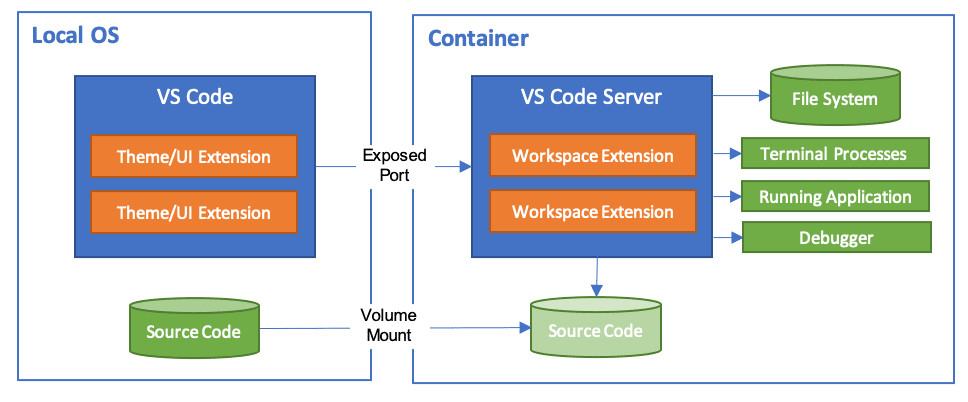
\includegraphics[width=0.9\textwidth]{assets/images/architecture-containers.png}
	\caption{Devcontainer Architecture: VS Code and Docker Integration \cite{DevelopingContainerUsing}}
\end{figure}

In this architecture, Visual Studio Code, running on the local machine, provides the
interface for the developer to interact with the container. The local machine runs
UI-related extensions such as themes, while the container hosts the VS Code server
and manages all the runtime tasks.
Inside the container, developers have access to
the file system, terminal processes, application runtimes, and debugging capabilities.
The workspace files, including the source code, are mounted from the local system
into the container using a volume mount, allowing seamless interaction with the code
from within the container. Exposed ports allow services running inside the container,
such as web servers, to be accessed from the local machine.

This setup ensures a local-quality development experience while providing all the
benefits of containerized isolation. Developers can perform tasks such as
code navigation, IntelliSense, and debugging without worrying about conflicts with
local environments. Visual Studio Code can run in two primary modes with Dev Containers:
as a full-time development environment inside the container, or by attaching to a
pre-existing running container for inspection or debugging purposes.

By leveraging Dev Containers, developers can ensure a consistent, isolated development
workflow while benefiting from the reproducibility and portability that Docker containers
offer. This integration streamlines the process of setting up a development environment,
making it easier to manage complex dependencies and configurations in a unified,
containerized workspace.

\subsubsection{Devcontainer Setup for Development Environments}

The Devcontainer setup used for this application highlights the power of
containerization technologies in creating a consistent and isolated development
environment. The setup consists of three key files: \texttt{devcontainer.json},
\texttt{Dockerfile}, and \texttt{.vscode/extensions.json}. Together, these files
configure the containerized development environment, providing developers with all
the necessary tools and dependencies without affecting the host system. By using a
container, the development environment remains reproducible across different machines,
ensuring consistency throughout the project lifecycle. Although this example uses
Visual Studio Code Dev Containers, the underlying principles of containerization—such
as environment isolation and dependency management—remain relevant across different
tools and technologies.

The \texttt{devcontainer.json} file is the cornerstone of this setup. It defines
how the development container is built and managed, specifying important parameters
such as the Dockerfile location, port forwarding, and workspace mounting. The following
is the configuration used for the Rust project:

\begin{lstlisting}[caption={devcontainer.json Configuration}]
{
  "name": "Rust Development Container",
  "build": {
    "dockerfile": "Dockerfile",
    "context": ".."
  },
  "forwardPorts": [
    8000
  ],
  "mounts": [
    "source=${localWorkspaceFolder},target=/app,type=bind"
  ]
}
\end{lstlisting}


This file defines several key aspects of the containerized environment. The
\texttt{dockerfile} attribute specifies the Dockerfile used to build the container,
while the \texttt{context} is set to the parent directory. This allows Docker to
access all the files needed to construct the environment. The \texttt{forwardPorts}
section ensures that port 8000 from within the container is accessible on the host
system, facilitating local testing of web applications. Finally, the \texttt{mounts}
section binds the local workspace folder to the \texttt{/app} directory within the
container, ensuring that changes made on the host machine are immediately reflected
inside the container. In this setup, the local workspace directory, represented
by the \texttt{\${localWorkspaceFolder}} variable, is bound to the \texttt{/app}
directory inside the container

The \texttt{Dockerfile} is used to create the containerized environment. In this
case, the Dockerfile is designed specifically for development purposes, optimizing
for flexibility and ease of use rather than production deployment. It defines the
base environment, installs necessary tools, and configures additional settings that
are critical for Rust development. Below is the Dockerfile used in this project:

\begin{lstlisting}[caption={Development Dockerfile for Rust Project}]
FROM rust:1.80.1-slim-bullseye

ENV DEBIAN_FRONTEND=noninteractive
ENV SHELL=/bin/bash
ENV PATH="/root/.proto/bin:$PATH"

RUN apt-get update && \
  apt-get install -y --no-install-recommends \
  git=1:2.30.2-1* \
  gzip=1.10-4* \
  unzip=6.0-26* \
  xz-utils=5.2.5-2.1* \
  curl=7.74.0-1.3* \
  pkg-config=0.29.2-1* \
  openssl=1.1.1* \
  libssl-dev=1.1.1* \
  musl-tools=1.2.2-1* \
  make=4.3-4.1* \
  && \
  apt-get clean && \
  rm -rf /var/lib/apt/lists/*

SHELL ["/bin/bash", "-o", "pipefail", "-c"]

RUN curl -fsSL https://moonrepo.dev/install/proto.sh | \
    bash -s -- 0.40.4 --yes && \
    proto plugin add moon \
    "https://raw.githubusercontent.com/moonrepo/moon/master/proto-plugin.toml" && \
    proto install moon

WORKDIR /app

COPY .moon .moon
COPY .prototools .prototools
COPY dockerManifest.json dockerManifest.json
COPY moon.yml moon.yml

RUN moon docker setup && \
    cargo install cargo-watch --locked
\end{lstlisting}

The Dockerfile begins by using the official Rust image \texttt{rust:1.80.1-slim-bullseye},
which ensures that the Rust toolchain is available within the container. Key environment
variables are defined to streamline the package installation process and configure the
shell. A series of packages are installed using \texttt{apt-get}, including Git, OpenSSL,
and \texttt{pkg-config}, which are necessary for building and testing Rust applications.

Next, the \texttt{moonrepo} tool is installed via the Proto installer, a tool used to
manage project workflows and tasks. This enables the environment to manage project tasks
efficiently. The Dockerfile also sets the working directory to \texttt{/app}, where the
local workspace is mounted. Various configuration files, such as \texttt{moon.yml} and
\texttt{dockerManifest.json}, are copied into the container. Lastly, the \texttt{moon}
tool is configured, and \texttt{cargo-watch} is installed to monitor file changes,
providing a productive development experience with real-time feedback.

The \texttt{.vscode/extensions.json} file specifies the recommended editor extensions
to install in Visual Studio Code. This
ensures that all developers have the required tools within the IDE to interact with
the containerized environment effectively. Below is the configuration used for this
project:

\begin{lstlisting}[caption={Recommended VS Code Extensions}]
{
    "recommendations": [
        "rust-lang.rust-analyzer",
        "ms-azuretools.vscode-docker",
        "ms-vscode-remote.remote-containers",
        "moonrepo.moon-console"
    ]
}
\end{lstlisting}

This file recommends several key extensions for Rust development and for Docker
management, the \texttt{remote-containers} extension is necessary
to enable Visual Studio Code to interact
with the container. The \texttt{moon-console} extension integrates with the Moonrepo
tool, allowing developers to manage project workflows directly within the editor.

Together, these files create a complete, containerized development environment that
ensures consistency across different machines. The environment is isolated from the
host system, yet remains fully integrated with the developer's workflow through Visual
Studio Code. The setup provides a robust solution for managing dependencies, building
and testing Rust applications, and handling project tasks within a containerized
environment.
